\documentclass[11pt]{beamer}
\usetheme{Antibes}
\usepackage[utf8]{inputenc}
\usepackage[german]{babel}
\usepackage[T1]{fontenc}
\usepackage{amsmath}
\usepackage{amsfonts}
\usepackage{amssymb}
\usepackage{graphicx}
\author{Gruppe C14 \\ Julián Häck, Martin Koytek, Lars Wenning, Erik Zimmermann}
\title{Messung der Schallgeschwindigkeit über Variation der Resonanzfrequenzen}
\begin{document}

\section{Versuchsbeschreibung}
\begin{frame}
\begin{equation}
f_n = \frac{n\cdot v}{2\cdot L}
\end{equation}
\begin{itemize}
\item grob die Resonanzfrequenzen vermessen
\item danach an den Resonanzfrequenzen mit deutlich mehr Messpunkten messen
\end{itemize} 
\end{frame}

\section{Aufbau und Durchführung}
\begin{frame}{Aufbau}
\begin{figure}[H]
\centering
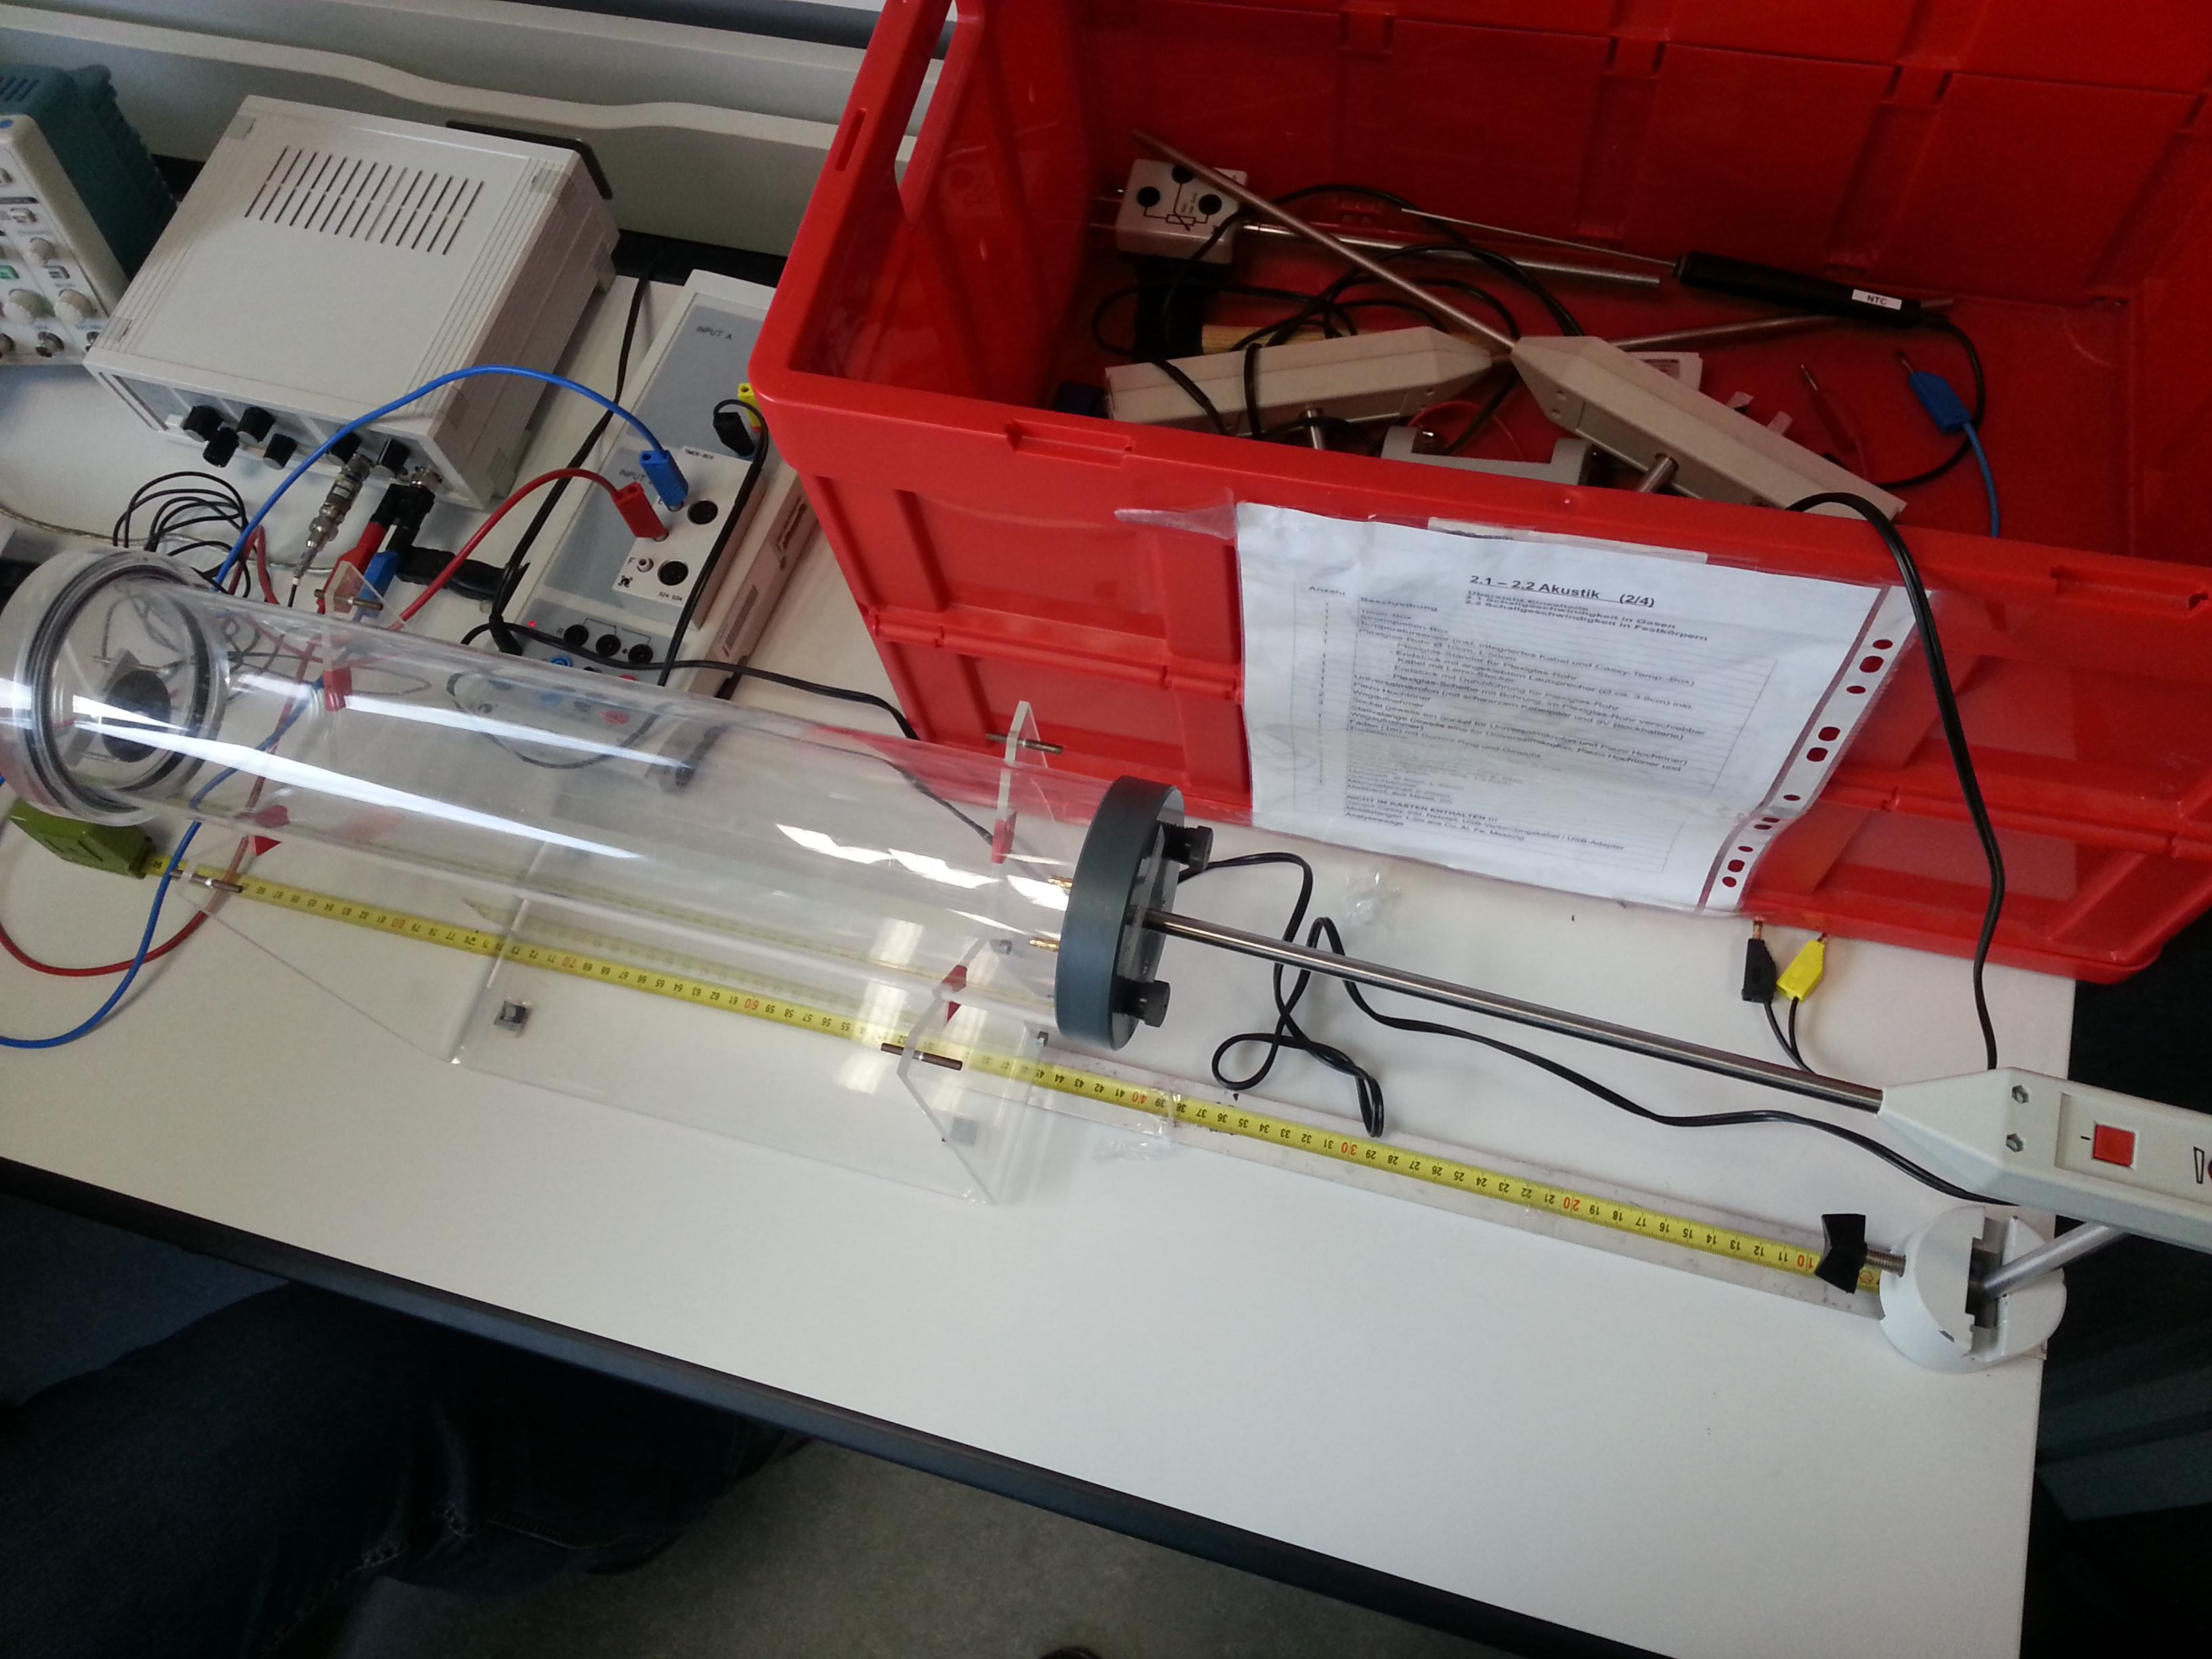
\includegraphics[scale=0.1]{Bilder/Frequenzvariation3.jpg}
\caption{Versuchsaufbau zur Messung der Schallgeschwindigkeit durch Variation der Resonanzfrequenzen}
\end{figure}
\end{frame}

\begin{frame}{Durchführung}
\begin{figure}[H]
\centering
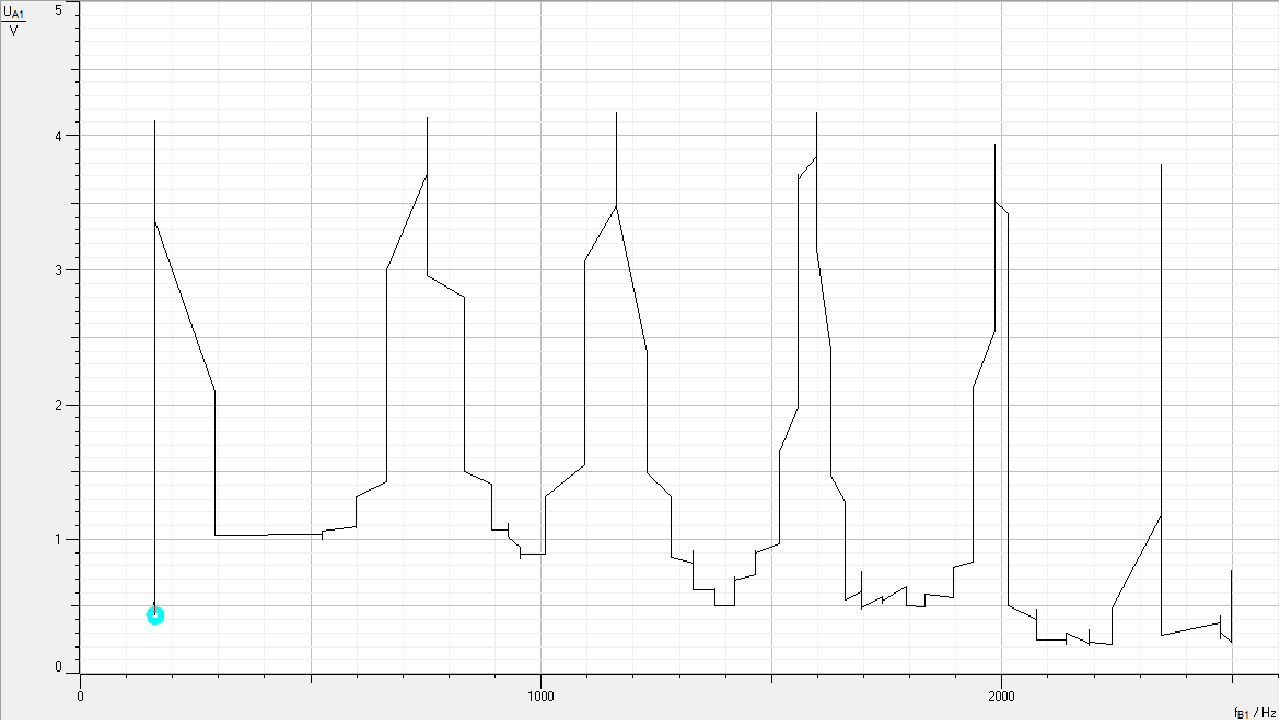
\includegraphics[scale=0.3]{Bilder/grobevermessung.png}
\caption{Grobe Vermessung der Resonanzfrequenzen - die deutlich ausgeprägten Peaks werden später genauer untersucht.}
\end{figure}
\end{frame}

\begin{frame}{Durchführung}
\begin{figure}[H]
\centering
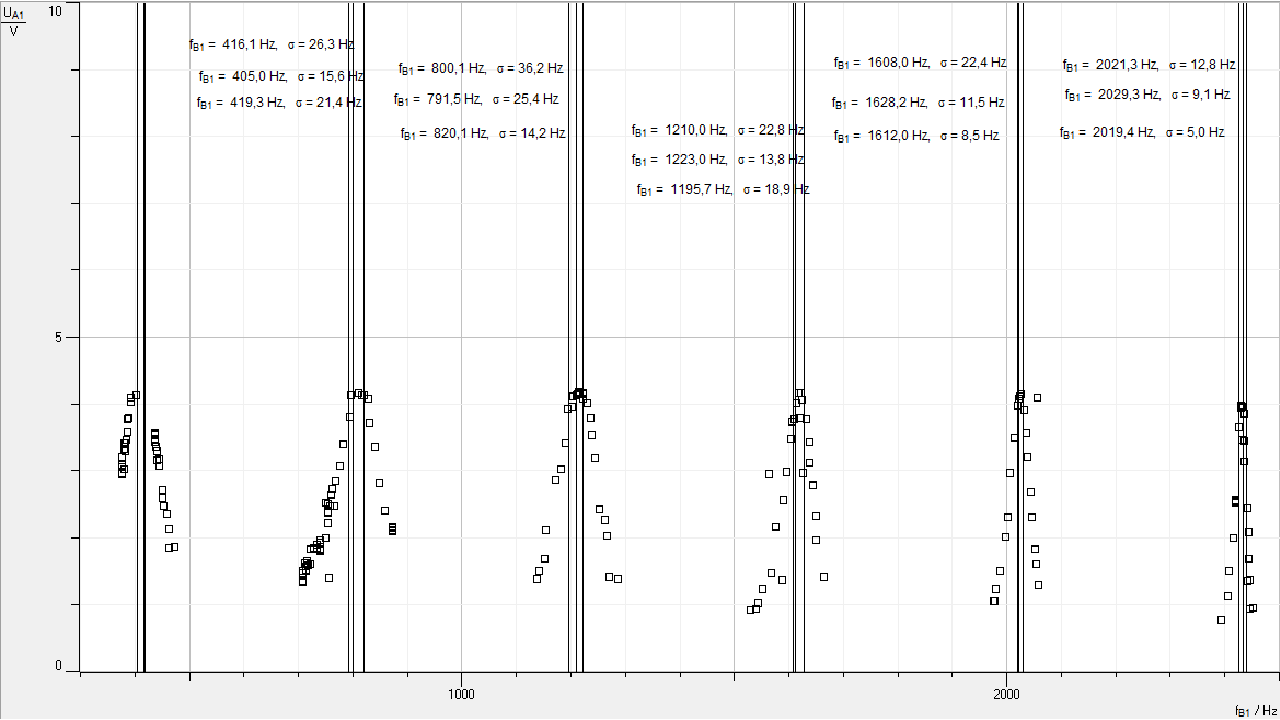
\includegraphics[scale=0.3]{Bilder/vermessung_variation_genau.png}
\caption{genaue Vermessung der Peaks an einer Beispiel Messung}
\end{figure}
\end{frame}

\section{Auswertung}
\begin{frame}{Rohdaten}
\begin{table}[H]
\begin{tabular}{c|c|c|c|c|c|c}
vermutete Res F & 400 & 800 & 1200 & 1600 & 2000 & 2400 \\ 
\hline 
Peak I & 416.0 & 822.5 & 1210.0 & 1608.0 & 2031.1 & 2433.4 \\  
$asym_r$ Peak I & 417.0 & 826.8 & 1212.6 & 1629.6 & 2041.4 & 2443.7 \\  
$asym_l$ Peak I & 404.9 & 798.2 & 1190.0 & 1573.9 & 2019.3 & 2425.5 \\ 
\hline 
Peak II & 420.7 & 822.1 & 1210.9 & 1620.0 & 2037.2 & 2446.7 \\  
$asym_r$ Peak II & 423.0 & 836.4 & 1216.5 & 1631.3 & 2047.8 & 2467.3 \\ 
$asym_l$ Peak II & 404.3 & 797.5 & 1194.0 & 1612.3 & 2013.8 & 2421.3 \\ 
\hline 
Peak III & 416.1 & 800.1 & 1210.0 & 1612.0 & 2019.4 & 2433.4 \\  
$asym_r$ Peak III & 419.3 & 820.1 & 1223.0 & 1628.2 & 2029.3 & 2439.2 \\  
$asym_l$ Peak III & 405.0 & 791.5 & 1195.7 & 1608.0 & 2019.4 & 2425.5
\end{tabular}
\caption{Vermessung der Resonanzfrequenzen, wobei $asym_r$ und $asym_l$ die asymmetrische Peakvermessung in Cassy (alle Angaben in Hz)} 
\end{table}
\end{frame}

\begin{frame}{Transformation der Rohdaten}
\begin{table}[H]
\begin{tabular}{c|c|c|c|c|c|c}
verm Res F &400&800&1200&1600&2000&2400\\ 
\hline 
$\bar{M}$ & 412.92 & 812.80 & 1206.97 & 1614.70 & 2030.07 & 2437.33 \\ 
\hline 
$\sigma_{\bar{M}}$ & 6.94 & 16.00 & 11.16 & 18.21 & 10.90 & 14.32 \\ 
\end{tabular}
\caption{Mittelwerte und deren Fehler (alle Angaben in Hz)} 
\end{table}
\end{frame}

\begin{frame}{Transformation der Rohdaten}
\begin{figure}[H]
\centering
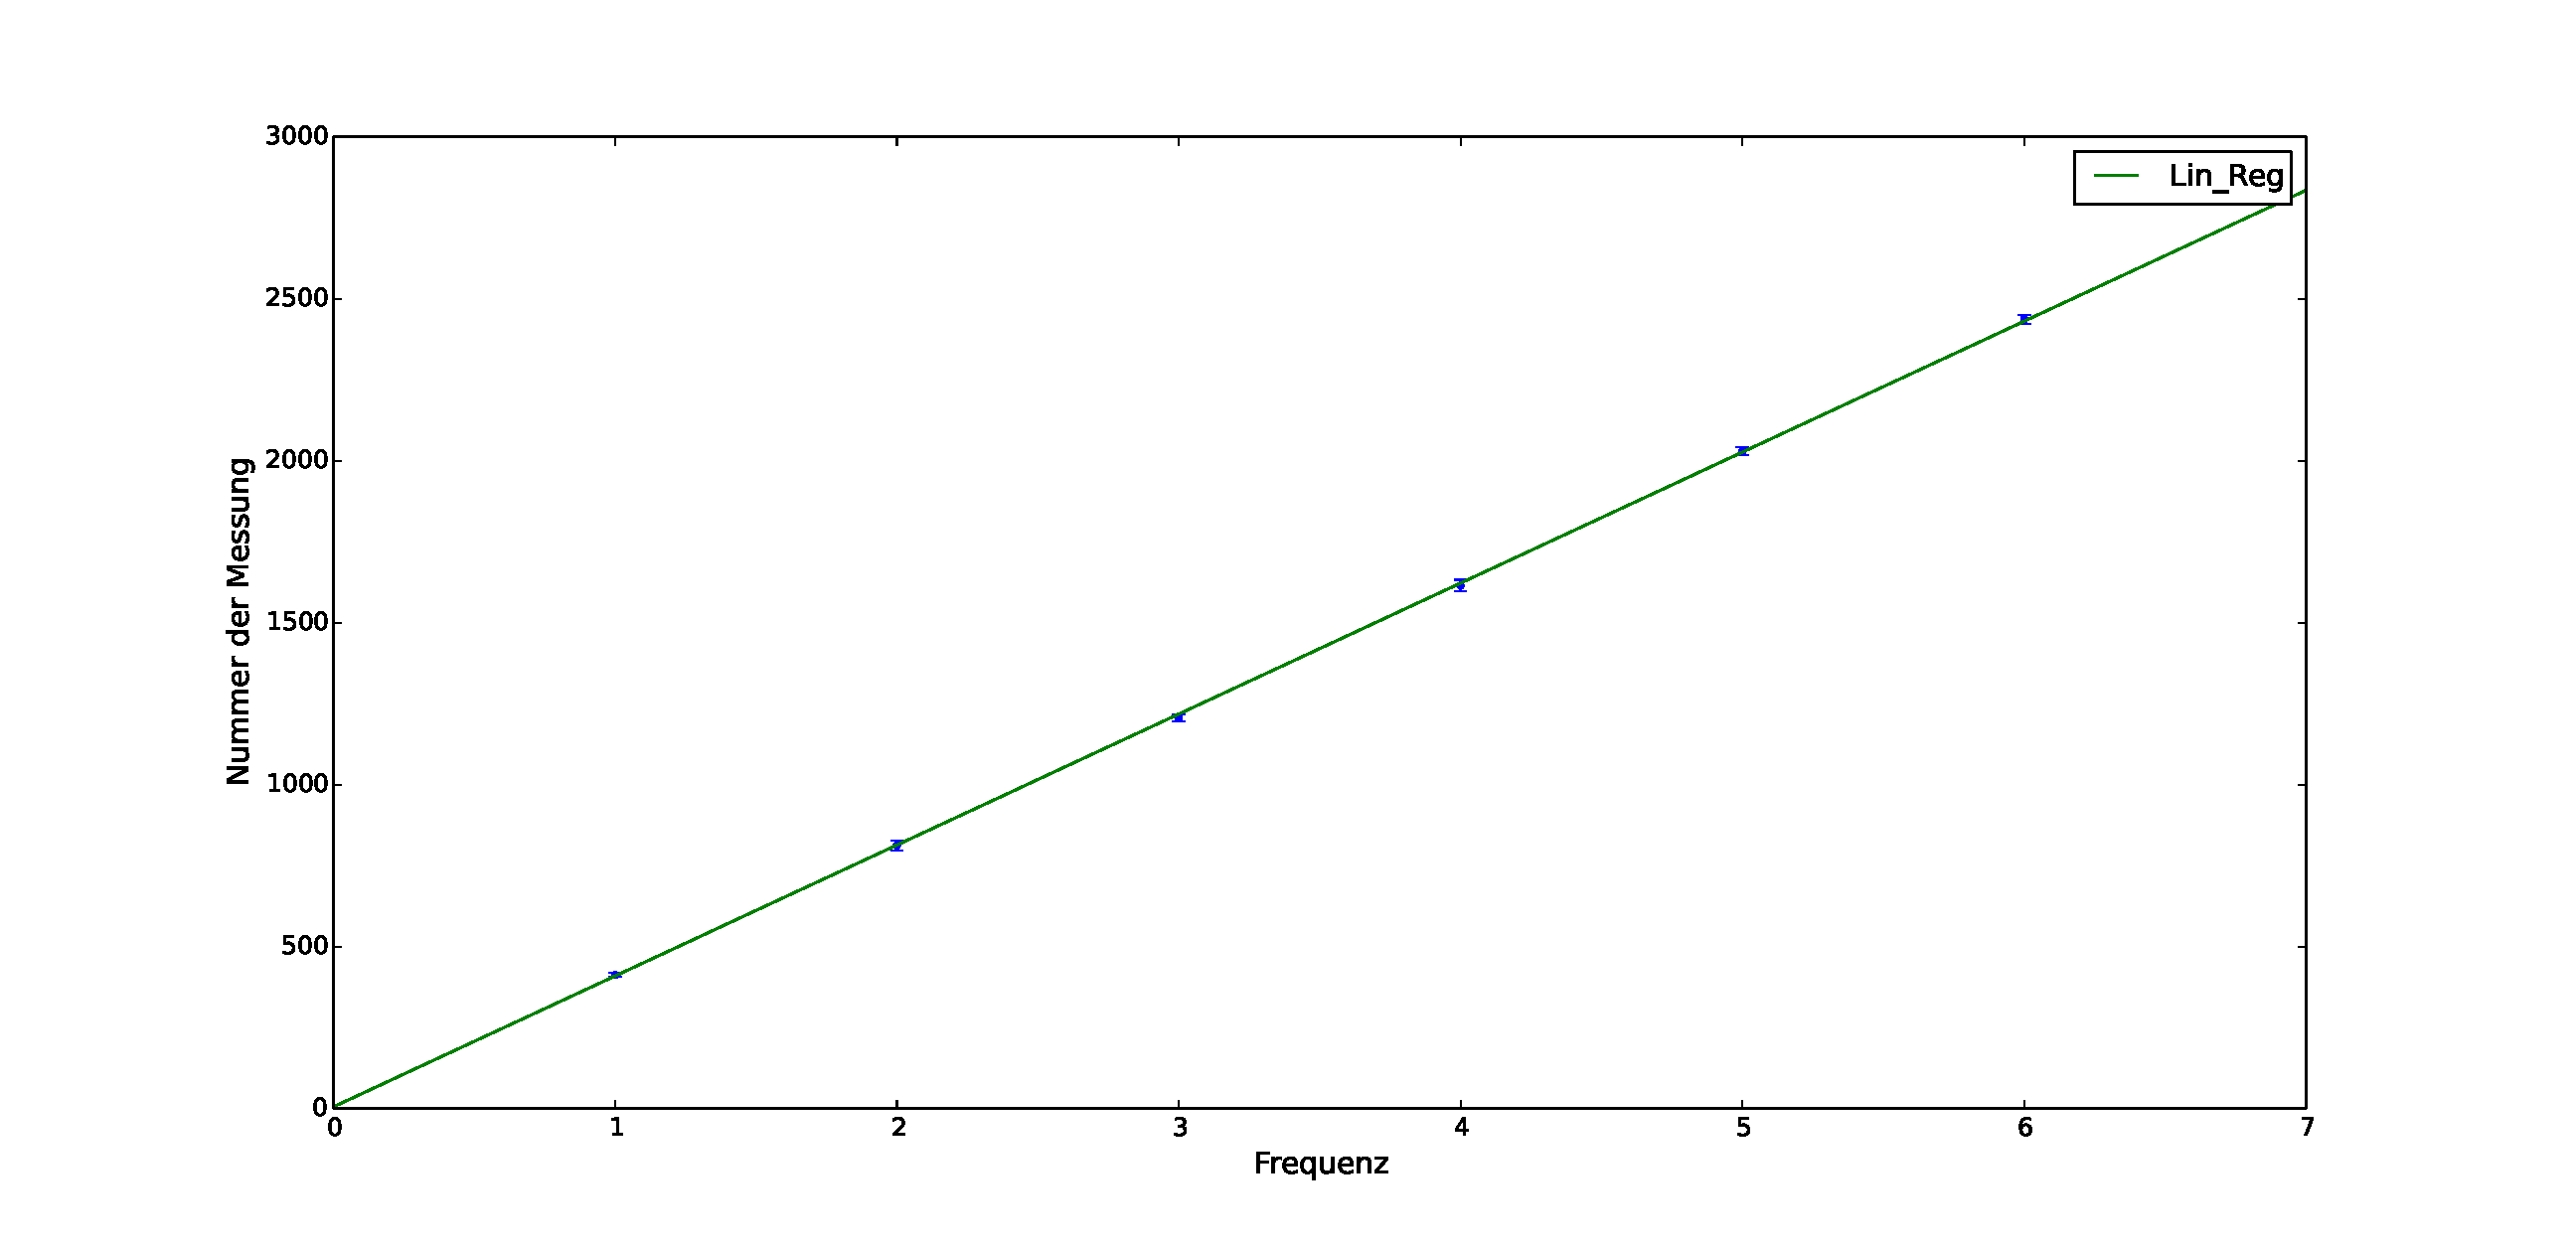
\includegraphics[scale=0.25]{Bilder/linreg_variation.eps}
\caption{Lineare Regression, die Steigung gibt $\frac{v_{Schall}}{2\cdot L}$ zurück, $\frac{\chi^2}{f} = 0.43$}
\end{figure}
\end{frame}

\begin{frame}{Auswertung der Transformation}
\begin{figure}[H]
\centering
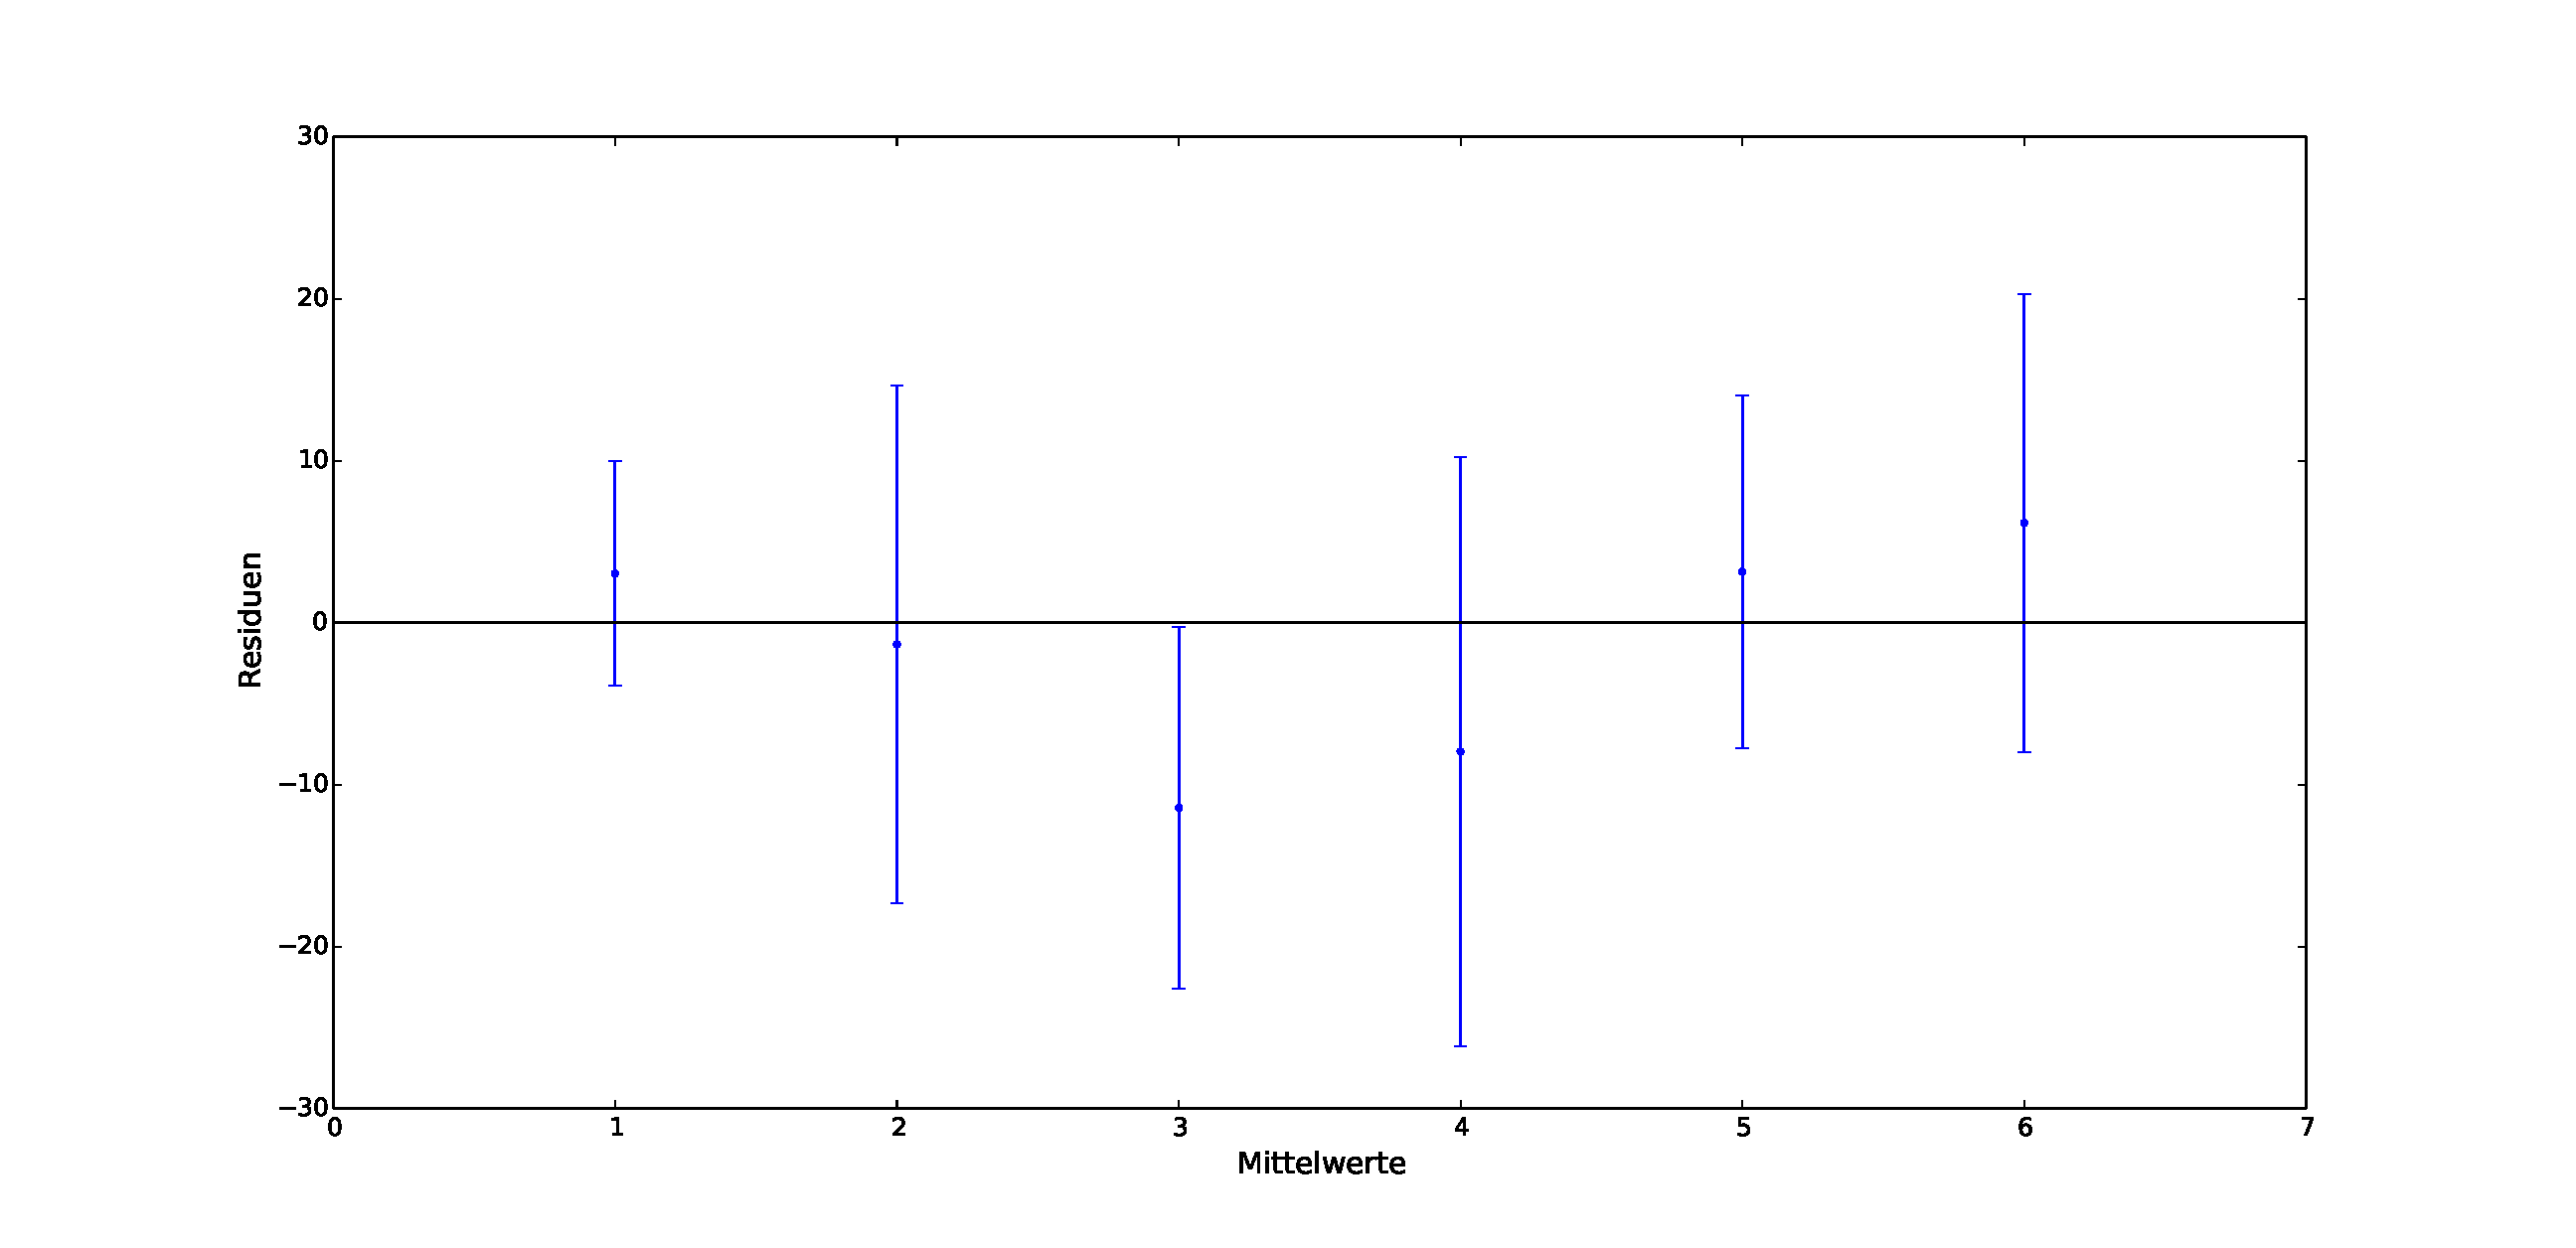
\includegraphics[scale=0.25]{Bilder/Residuen_Variation_Frequenzen.eps}
\caption{Residuenplot (Werte-Fit), zeigt Güte der Anpassung}
\end{figure}
\end{frame}

\begin{frame}{Fehlerrechnung und Ergebnis}
\begin{equation}
\sigma_v = \sqrt{f_R^2\cdot\sigma_{\lambda}^2 + \lambda^2\cdot\sigma_f^2}
\end{equation}
mit
\begin{equation}
\sigma_{\lambda} = \sigma_{\bar{M}}\cdot\sqrt{2}
\end{equation}
$\bar{M}$ und $\sigma_{\bar{M}}$ haben wir erhalten durch:
\begin{equation}
\bar{M} = \frac{\sum_{i=1}^{N}{X_i}}{N}
\end{equation}
und
\begin{equation}
\sigma_{\bar{M}}=\frac{\sqrt{\frac{\sum_{i=1}^{N}({X_i-\bar{M}})^2}{N-1}}}{\sqrt{N}}
\end{equation}
Nach der Korrektur erhalten wir einen Wert für $v$ von
\begin{equation}
v = 343.46 \pm 2.08\,\frac{m}{s}
\end{equation}.
\end{frame}

\section{Fazit}
\begin{frame}{Fazit}
\begin{itemize}
\item unser Wert: $343.46 \pm 2.08\,\frac{m}{s}$
\item Literaturwert: $v_{lit}=343\,\frac{m}{s}$
\item $\Rightarrow 0.58\%$ Abweichung
\\
\item Güte unserer Anpassung: $\frac{\chi^2}{f} = 0.43$
\end{itemize}
\end{frame}

\end{document}